\chapter{Opis koncepcji rozwiązania i zastosowane metody biometryczne}
\label{ch:koncepcja}

\section{Ogólna idea działania systemu}
Zaprojektowany system opiera się na symulacji skanera biometrycznego, który został zintegrowany z desktopową aplikacją recepcyjną napisaną w technologii WPF. Aplikacja współpracuje z relacyjną bazą danych MySQL, w której przechowywane są zarówno dane użytkowników, jak i przetworzone dane biometryczne.

Działanie modułu biometrycznego w aplikacji zostało podzielone na dwa główne procesy oraz przedstawione w formie schematu na rysunku \ref{idea_biometryka}.
\begin{enumerate}
    \item \textbf{Rejestracja (Enrolment)} -- proces dodawania i przypisywania wzorców biometrycznych do kont użytkowników. Pracownik recepcji za pomocą dedykowanego okna menedżera wskazuje pliki graficzne reprezentujące próbki odcisków palców klienta. Aplikacja wczytuje obraz, a dedykowany moduł kryptograficzny oblicza dla niego hasz (aHash). Zarówno oryginalny obraz (zapisany jako obiekt typu \texttt{LONGBLOB}), jak i wyliczony skrót w postaci szesnastkowej, trafiają do bazy danych z powiązaniem do odpowiedniego identyfikatora użytkownika. Każdy użytkownik może mieć maksymalnie 3 wzorce biometryczne w bazie.
    \item \textbf{Identyfikacja (1:N)} -- proces weryfikowania tożsamości klienta podczas wejścia na obiekt. Podczas skanowania, system przyjmuje nową próbkę biometryczną i w czasie rzeczywistym generuje dla niej analogiczny skrót aHash. Następnie skrót ten jest zestawiany ze wszystkimi wpisami w bazie danych w poszukiwaniu najlepszego dopasowania. Po przekroczeniu ustalonego progu pewności (82\%), system autoryzuje wejście, wyświetla profil klienta i automatycznie loguje czas rozpoczęcia lub zakończenia jego wizyty.
\end{enumerate}

\begin{figure}[H]
    \centering
    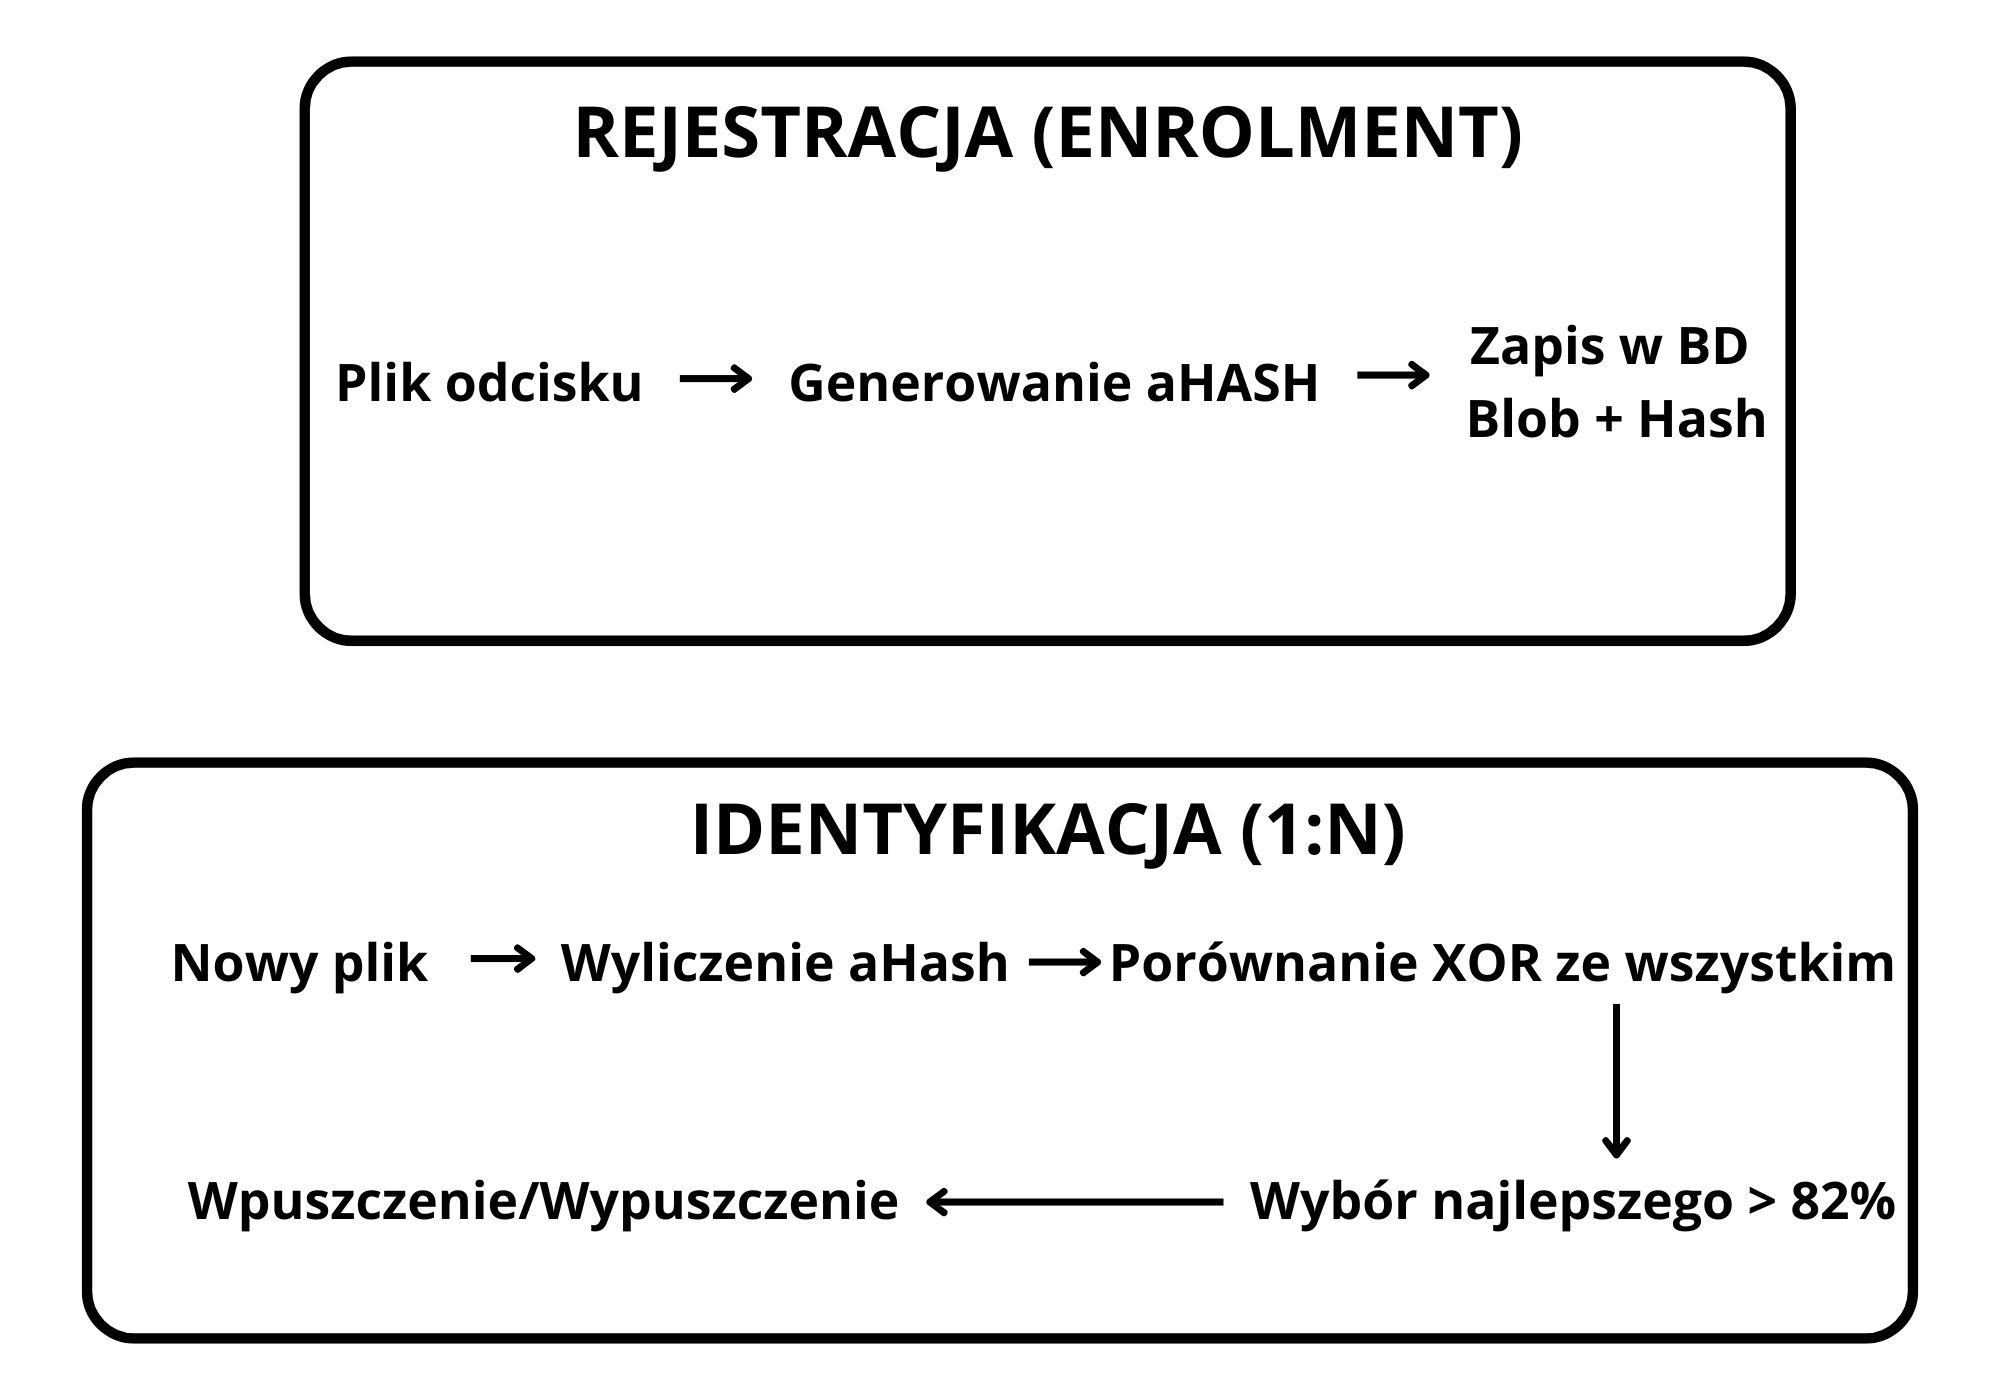
\includegraphics[width=0.7\linewidth]{figures/idea_biometryka.png}\\
    \caption{Schemat ogólnego działania systemu.\label{idea_biometryka}}
\end{figure}

\section{Schemat blokowy przetwarzania danych}
Proces przetwarzania danych biometrycznych od momentu załadowania próbki przez symulowany czytnik aż po decyzję o autoryzacji jest przedstawiony na schemacie \ref{schemat_biometryka}:

\begin{figure}[H]
    \centering
    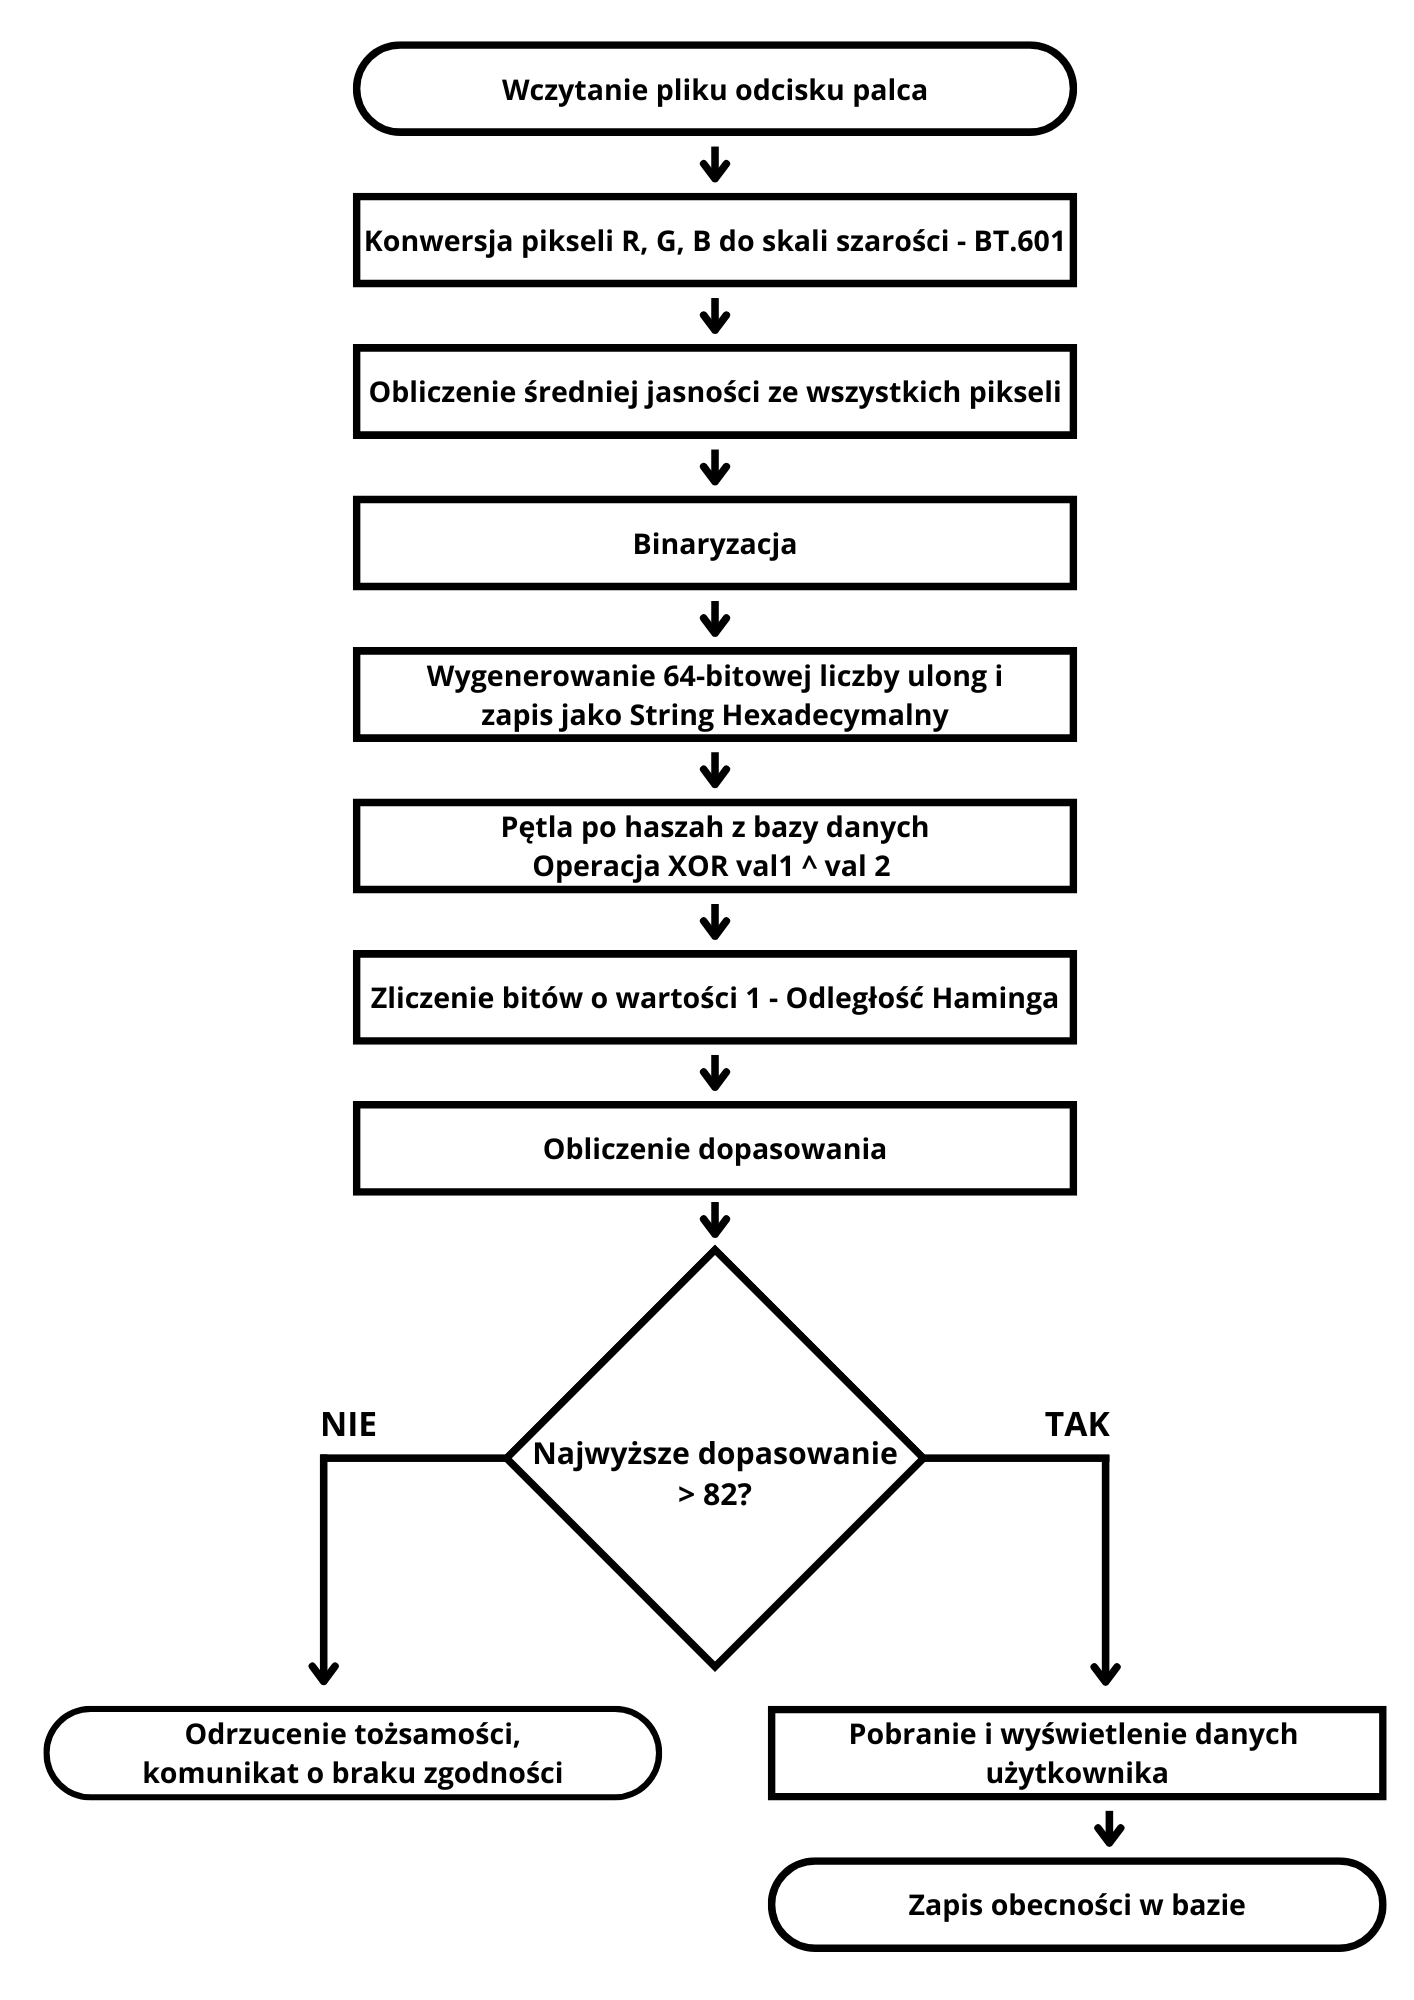
\includegraphics[width=0.7\linewidth]{figures/schemat_biometryka.png}\\
    \caption{Schemat blokowy przetwarzania danych biometrycznych.\label{schemat_biometryka}}
\end{figure}

\section{Zastosowane metody i algorytmy}
W systemie zrezygnowano z tradycyjnych funkcji skrótu (np. MD5 czy SHA), ponieważ najmniejsza zmiana obrazu (wynikająca np. z szumu sensora lub innego przyłożenia palca) generowałaby zupełnie inny wynik. Co zaprzeczało by założeniom systemu. Zamiast tego zastosowano algorytmy odporne na drobne zniekształcenia.

\subsection{Percepcyjne Haszowanie Obrazu (aHash)}
System wykorzystuje technikę haszowania Average Hash\cite{HackerFactorAverageHash} (aHash), która opiera się na analizie ogólnej struktury obrazu. Zamiast polegać na dokładności co do piksela, w metodzie aHash redukuje się obraz do rozmiarów 8x8 pikseli, co skutkuje pozostawieniem jedynie wyraźnych cech wizualnych (ogólnego zarysu linii papilarnych). W następnym kroku odbywa się konwersja do odcieni szarości\cite{TarasiukGFK} zgodnie ze wzorem fizjologicznej czułości oka:
\begin{equation}
    \text{Luminancja} = R \cdot 0.299 + G \cdot 0.587 + B \cdot 0.114
\end{equation}
Średnia jasność staje się następnie progiem filtru binaryzującego. Wynikiem działania algorytmu jest kompaktowa, 64-bitowa sygnatura numeryczna, która reprezentuje wizualny rozkład jasności próbki.

\subsection{Odległość i waga Hamminga w weryfikacji 1:N}
Proces identyfikacji w czasie rzeczywistym wymaga wysokiej wydajności. W tym celu zastosowano operacje bitowe służące do wyznaczania odległości Hamminga\cite{HammingDistanceDataCamp}, definiowanej jako liczba różniących się bitów pomiędzy dwiema sygnaturami o tej samej długości. W implementacji wykorzystano różnicę symetryczną (XOR) dla obu porównywanych zmiennych typu \texttt{ulong}. Zliczanie ilości zapalonych bitów w wyniku tej operacji (tzw. Hamming Weight) pozwala szybko ocenić stopień podobieństwa wzorców.
Procentowe prawdopodobieństwo zgodności wylicza się ze wzoru:
\begin{equation}
    \text{Prawdopodobieństwo zgodności} = \left( \frac{64 - \text{dystans}}{64} \right) \cdot 100\%
\end{equation}

\subsection{Uzasadnienie wyboru zastosowanych metod}
Wybór metody aHash w zestawieniu z modelem operacji bitowych zoptymalizował koszty wdrożeniowe:
\begin{itemize}
    \item \textbf{Szybkość:} W przeciwieństwie do metod uczenia maszynowego, zastosowane algorytmy nie wymagają dodawania obszernych bibliotek, posiadania sprzętowych akceleratorów AI, ani czasochłonnego treningu. Identyfikacja działa szybko, nie blokując operacji interfejsu użytkownika.
    \item \textbf{Elastyczność weryfikacyjna:} Ustalenie progu akceptacji na poziomie 82\% (dopuszczenie maksymalnie 13 różniących się bitów na 64) zapewnia odporność na zmienność próbek. Pozwala to na uniknięcie problemu częstego, błędnego odrzucania użytkowników w przypadku nierównego nacisku palca, zanieczyszczeń na skanerze lub przesuszenia/uszkodzenia skóry, utrzymując jednocześnie bardzo niski współczynnik błędnej akceptacji.
\end{itemize}
